\section{Science on the International Space Station} \label{science-on-the-international-space-station}

\subsection{Why tell our story?} \label{why-tell-our-story}
There are lots of papers, reports, blogs and general writing on space, NASA, and science. So why write more?
\emph{Because very, very few people actually understand how science experiments are conducted, from start to finish, either in the lab, or onboard the on-orbit laboratory of the International Space Station (ISS).}
My aim here to tell the story of how science actually works, for a broad audience:
\begin{itemize}
\item the general tax-paying public who wants to know more about what is going on in NASA
\item NASA staff who may be deeply knowledgable about a small part of the process, but don't get a good overview---and who want to hear directly from the Principal Investigators (scientists)
\item policy folks who want a deeper view of what we do, beyond what can be described in a report
\item the astronaut crew on  we work with, who want a direct line to what we are doing
\end{itemize}

I intend this to be a cross-breed of a blog, textbook, collection of essays and
technical manual. Some of the posts will give the nitty-gritty \emph{in medias
res} narrative of what we are doing on a day-to-day basis. Other entries will
summarize previous knowledge to give an historical context to the work we are
doing. Still others may dive a little deeper into the technical details of the
tools we are using, hardware and software, both to do the science and
communicate its results. I hope to cover a broad range:
\begin{itemize}
\item The scientific background of experiments that precede and motivate ours
\item What we are actually trying to understand in our current experiment
\item How we prepare and characterize our experimental samples
\item What instrumentation and laboratory apparatus we use, on the ground and in orbit
\item The process of packaging and launching our samples to the ISS
\item Conducting on-orbit experiments in collaboration with the astronaut crew
\item The raw data and how we process it
\item How our analysis leads to the scientific story we will tell through papers and presentations
\item Writing a scientific paper
\item Preparing a scientific talk (and possibly its presentation)
\end{itemize}

\subsection{Opening up the process of doing science}\label{opening-up-the-process-of-doing-science}
I aim to be maximally open throughout. This means posting raw data when
feasible, the actual computer code we use for the analysis (and potentially
giving a way for you all to play with the data and code yourself in an
interactive environment---stay tuned), early drafts of the paper as we write it,
and maybe our presentation drafts before they are delivered.

My commitment here is to make as much of our work accessible directly to anyone
to tinker with: open-source software, open-access publications, but also free,
open access to the raw data; even this website itself, hosted on Github, is
completely open---not just the text, but the entire revision history, and the
code that runs it. So please download, play around, make your own modifications,
and let us know through the comments what you think and if you found something
new that we might have missed. This is a different way of doing science that
takes advantage of a lot of the new information-based technologies that were not
available in years past, and the way I think science should be done. I will
elaborate more on the motivation and tools in a later post.
\subsection{Who am I?}\label{who-am-i}
\begin{figure}
\begin{center}
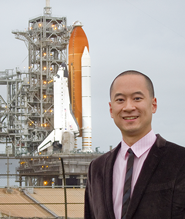
\includegraphics[width=2in]{./images/peterlu_atlantis_launchpad_sm_110707.png}
\end{center}
\caption{Launchpad photo}
\end{figure}

I am a physicist at Harvard, currently serving in a staff position known as a
post-doctoral fellow, meaning I continue to do research after receiving my PhD.
I am funded by {NASA} directly through a research
grant to my official employer, {Harvard University}
(Cambridge, MA), which broadly-speaking supports the scientific aspects of our
work. I also receive some additional support as a subcontractor to assist with
the engineering aspects, helping to develop and test the hardware and software,
of the experiment by working closely with the main NASA contractor,
{ZIN Technologies} (Cleveland, OH). More
information on me and my work can be found on my webpage,
{peterlu.org}. I act independently, and represent
my own views here. Though I am employed by Harvard, they do not control (pretty
much ever) what any of us say or do. NASA, similarly, gives a research grant and
is not able (as much as they sometimes would like) to be able to control what
its funding recipients can say. ZIN is contracted to engineer, deploy and run
complex instrumentation and serves in a technical capacity, and does not appear
to have much of a corporate message to spread beyond NASA.

I do anticipate some fraction of what I write to disagree with the perspectives
of others; if 80\% of the readers agree with me 80\% of the time, then that to
me is a healthy balance that still leaves room for new ideas to develop and be
fleshed out in a congenial manner. If you think I am a little off-base, please
leave some respectful comments and I will do my best to respond in a timely
fashion (though note that I will moderate and delete anything offensive,
off-topic, spam, or irrelevant).

Hopefully we have an interesting and informative journey, and do some great
science along the way!

